\documentclass[11pt,a4paper]{article}
\usepackage[T1]{fontenc}
\usepackage[utf8]{inputenc}
\usepackage{lmodern}
\usepackage[margin=2.5cm]{geometry}
\usepackage{booktabs}
\usepackage{tabularx}
\usepackage{array}
\usepackage{longtable}
\usepackage{xcolor}
\usepackage{enumitem}
\usepackage{fancyhdr}
\usepackage{titlesec}
\usepackage{listings}
\usepackage{float}
\usepackage{amssymb}
\usepackage{tikz}
\usetikzlibrary{positioning,arrows.meta,calc,decorations.pathreplacing}
\usepackage{xurl}
\usepackage{hyperref}

\hypersetup{colorlinks=true, linkcolor=blue!50!black, urlcolor=blue!50!black}

\definecolor{codebg}{gray}{0.96}
\definecolor{notebg}{RGB}{255,246,228}
\definecolor{noteframe}{RGB}{200,110,0}
\definecolor{tipbg}{RGB}{232,242,252}
\definecolor{tipframe}{RGB}{42,120,214}
\definecolor{okgreen}{RGB}{0,120,60}
\definecolor{kw}{RGB}{0,70,150}
\definecolor{cm}{RGB}{90,110,90}

\lstdefinelanguage{VHDLx}{
  morekeywords={library,use,entity,is,port,in,out,inout,end,architecture,of,begin,signal,constant,variable,
    process,if,then,elsif,else,wait,until,for,loop,while,report,severity,assert,generic,map,type,function,
    return,package,body,when,others,downto,to,not,and,or,file,generate,exit,procedure},
  sensitive=false, morecomment=[l]{--}, morestring=[b]"}
\lstset{
  basicstyle=\ttfamily\small,
  backgroundcolor=\color{codebg},
  frame=single,
  rulecolor=\color{gray!40},
  breaklines=true,
  columns=fullflexible,
  keepspaces=true,
  showstringspaces=false,
  keywordstyle=\color{kw}\bfseries,
  commentstyle=\color{cm}\itshape,
  upquote=true
}

\newcommand{\code}[1]{\texttt{#1}}
\newcommand{\bs}{\textbackslash\allowbreak{}}
\let\oldunderscore\_
\renewcommand{\_}{\oldunderscore\allowbreak{}}
\newcommand{\pld}[1]{\code{C:\bs PLD\bs #1}}
\newcommand{\menu}[1]{\textsf{#1}}
\newcommand{\checkbox}{$\square$\ }
\newcolumntype{Y}{>{\raggedright\arraybackslash}X}

\newcommand{\important}[1]{%
  \par\smallskip\noindent
  \fcolorbox{noteframe}{notebg}{\parbox{\dimexpr\linewidth-2\fboxsep-2\fboxrule\relax}{\small\textbf{Important.} #1}}%
  \par\smallskip}
\newcommand{\tip}[1]{%
  \par\smallskip\noindent
  \fcolorbox{tipframe}{tipbg}{\parbox{\dimexpr\linewidth-2\fboxsep-2\fboxrule\relax}{\small\textbf{Tip.} #1}}%
  \par\smallskip}
\newcommand{\why}[1]{%
  \par\smallskip\noindent
  \fcolorbox{tipframe}{tipbg}{\parbox{\dimexpr\linewidth-2\fboxsep-2\fboxrule\relax}{\small\textbf{Why.} #1}}%
  \par\smallskip}
\newcommand{\say}[1]{%
  \par\smallskip\noindent
  \fcolorbox{okgreen}{green!5}{\parbox{\dimexpr\linewidth-2\fboxsep-2\fboxrule\relax}{\small\textbf{What to say.} #1}}%
  \par\smallskip}

\setlength{\emergencystretch}{3em}
\setlength{\parskip}{4pt}
\setlength{\parindent}{0pt}
\titleformat{\subsection}{\normalfont\large\bfseries}{\thesubsection}{1em}{}
\pagestyle{fancy}
\fancyhf{}
\lhead{\small TeraNova -- FPGA Acceleration}
\rhead{\small Vivado simulation guide -- K.~Janssen (4994817)}
\cfoot{\small\thepage}
\renewcommand{\headrulewidth}{0.4pt}

\begin{document}

\begin{titlepage}
\centering
\vspace*{3cm}
{\LARGE\bfseries Vivado Simulation Guide\par}
\vspace{0.5cm}
{\Large Everything you need to know to simulate\\VHDL designs with the Vivado simulator (XSim)\par}
\vspace{0.3cm}
{\large TeraNova -- FPGA Acceleration\par}
\vspace{2cm}
\begin{tabular}{@{}ll@{}}
\textbf{Author}   & Kai Janssen (4994817) \\
\textbf{Version}  & 5 November 2026 \\
\textbf{Tools}    & Vivado 2025.1.1 (Vivado simulator, XSim), Windows \\
\textbf{Companion}& \emph{Rung Simulation Guide} (the ladder in Vivado) \\
\end{tabular}
\vfill
{\small Based on the Vivado Design Suite User Guide: Logic Simulation (UG900, version 2025.1), the Vivado Tcl Command Reference (UG835) and hands-on experience with the TeraNova testbenches. References at the end.\par}
\end{titlepage}

\tableofcontents
\newpage

% ==================================================================
\section{How to use this guide}
% ==================================================================
This guide teaches the Vivado simulator from zero. It is written for the situation ``I have tried simulating in Vivado before and it never worked''. Read it in this order:

\begin{enumerate}[nosep]
  \item Section~\ref{sec:concepts}: what a simulation actually is in Vivado (three tools, three steps). Ten minutes, and most past problems become understandable.
  \item Section~\ref{sec:practice}: a complete practice run with a small counter. Do it once with your hands on the keyboard; it takes about 20 minutes.
  \item Sections~\ref{sec:tb}--\ref{sec:debug}: reference material, to read when you need it: writing testbenches, settings, the wave window, debugging.
  \item Section~\ref{sec:trouble}: the troubleshooting table. When something fails, start here.
  \item Section~\ref{sec:cheat}: a one-page cheat sheet.
\end{enumerate}

The practice files are in \pld{sim\bs vivado\bs practice}. The improvement-ladder simulation for the tutor meeting has its own guide (\emph{Rung Simulation Guide}).

\important{Simulation needs \textbf{no licence}. The node-locked licence on Badr's laptop is only needed for synthesis and implementation of the ZCU102 design. Behavioural simulation with XSim runs on any PC with Vivado 2025.1.1 installed.}

% ==================================================================
\section{The concepts in ten minutes}\label{sec:concepts}
% ==================================================================

\subsection{What a simulation is}
A simulation runs your HDL code on the PC instead of on the FPGA. A \emph{testbench} (an extra HDL file with no ports) creates the clock, the reset and the input stimulus, instantiates your design as the \emph{unit under test} (UUT) and, ideally, checks the outputs. The simulator calculates every signal over time; you look at the result in the \emph{wave window} and in the messages of the Tcl Console.

\subsection{The three steps}
Every Vivado simulation, from the GUI or from a script, consists of three separate programs (Figure~\ref{fig:flow}). When ``the simulation fails'', it always fails in one of these three, and the message tells you which one. Knowing this is the single most useful thing in this guide.

\begin{figure}[H]
\centering
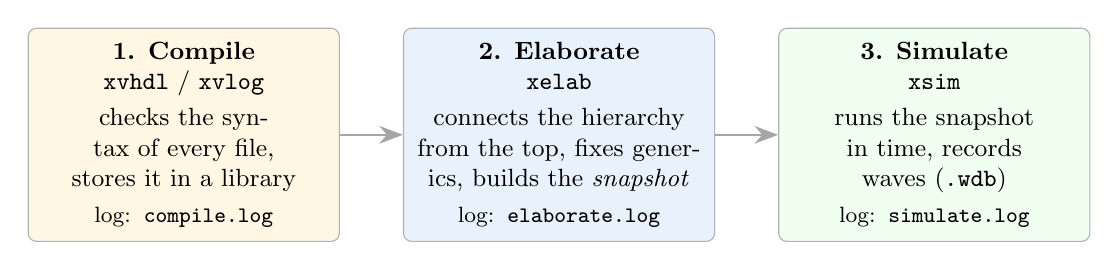
\begin{tikzpicture}[
  box/.style={draw=gray!60, rounded corners=3pt, fill=#1, align=center, text width=3.6cm, minimum height=2.3cm, inner sep=5pt, font=\small},
  arr/.style={-{Stealth[length=3mm]}, thick, gray!70}]
\node[box=notebg] (c) {\textbf{1. Compile}\\\code{xvhdl} / \code{xvlog}\\[2pt]checks the syntax of every file, stores it in a library\\[2pt]\footnotesize log: \code{compile.log}};
\node[box=tipbg, right=0.8cm of c] (e) {\textbf{2. Elaborate}\\\code{xelab}\\[2pt]connects the hierarchy from the top, fixes generics, builds the \emph{snapshot}\\[2pt]\footnotesize log: \code{elaborate.log}};
\node[box=green!6, right=0.8cm of e] (s) {\textbf{3. Simulate}\\\code{xsim}\\[2pt]runs the snapshot in time, records waves (\code{.wdb})\\[2pt]\footnotesize log: \code{simulate.log}};
\draw[arr] (c) -- (e);
\draw[arr] (e) -- (s);
\end{tikzpicture}
\caption{The three steps behind \menu{Run Simulation}. The logs are in \code{<project>.sim\bs sim\_1\bs behav\bs xsim}.}
\label{fig:flow}
\end{figure}

\begin{itemize}[nosep]
  \item \textbf{Compile} errors (\code{[VRFC 10-...]}) are language errors in a file: a typo, a missing library clause, VHDL-2008 code compiled as plain VHDL.
  \item \textbf{Elaborate} errors are about how the files fit together: the top cannot be found, a component has no matching entity, a port does not exist, a generic has the wrong type. In the GUI they appear as \code{[USF-XSim-62] 'elaborate' step failed}; the real message is in \code{elaborate.log}.
  \item \textbf{Simulate} problems are about behaviour: the run stops too early, signals stay \code{U} or \code{X}, an assertion fires, a file cannot be opened.
\end{itemize}

\subsection{Kinds of simulation}
\begin{tabularx}{\textwidth}{@{}lY@{}}
\toprule
\textbf{Kind} & \textbf{What is simulated} \\
\midrule
Behavioural (RTL) & Your HDL source code as written. Fast, full visibility. \textbf{This is what you use 95\,\% of the time, and what this guide is about.} \\
Post-synthesis functional & The synthesised netlist, without delays. Checks that synthesis understood your code. \\
Post-implementation timing & The placed and routed netlist with real delays (SDF). Slow; rarely needed when the design meets timing in static timing analysis. Needs the licensed implementation. \\
\bottomrule
\end{tabularx}

\subsection{Projects, filesets and simulation sets}
In a Vivado project the Sources window has three kinds of filesets:
\begin{itemize}[nosep]
  \item \textbf{Design Sources} (\code{sources\_1}): what is synthesised.
  \item \textbf{Constraints} (\code{constrs\_1}): XDC files; not used by simulation.
  \item \textbf{Simulation Sources} (\code{sim\_1}, \code{sim\_2}, \ldots): testbenches and simulation-only models. A simulation set normally also \emph{includes} the design sources, so you do not add your design twice.
\end{itemize}
A testbench belongs in \emph{Simulation Sources} only, so it is never synthesised. Every simulation set has its own \textbf{top} (shown in bold in the Sources window). You can have several simulation sets, for example one per testbench; the \emph{active} one (right-click \menu{Make Active}) is the one \menu{Run Simulation} uses.

\subsection{Libraries}
Every compiled VHDL unit lives in a \emph{library}. In a project the default library is \code{xil\_defaultlib}, and the VHDL name \code{work} always means ``the library this file is compiled into''. You rarely change this, but it is the clean way to have two different versions of an entity with the same name in one simulation: put each version in its own library (the ladder simulation does exactly this). AMD's own libraries (\code{unisim}, \code{xpm}, the IP libraries) come precompiled for XSim; \code{compile\_simlib} is only needed for third-party simulators such as Questa.

\subsection{The run folder}
The GUI writes everything for a behavioural run of \code{sim\_1} into
\[\code{<project>.sim\bs sim\_1\bs behav\bs xsim\bs}\]
The simulator also \emph{runs} in this folder. Two consequences:
\begin{itemize}[nosep]
  \item the three logs (\code{compile.log}, \code{elaborate.log}, \code{simulate.log}) and the scripts Vivado generated (\code{compile.bat}, \code{elaborate.bat}, \code{simulate.bat}, \code{*.prj}) are here: the first place to look when something fails;
  \item a relative file name in VHDL (\code{file\_open(f, "data.txt", ...)}) is relative to \textbf{this folder}, not to your source folder. This is the most common reason why a testbench that reads a file ``cannot find'' it (Section~\ref{sec:files}).
\end{itemize}

% ==================================================================
\section{Practice run: a counter from start to finish}\label{sec:practice}
% ==================================================================
This exercise uses two small files that are already on your PC:
\pld{sim\bs vivado\bs practice\bs counter.vhd} (the design) and \pld{sim\bs vivado\bs practice\bs tb\_counter.vhd} (the testbench). Both are listed in Appendix~\ref{app:practice}.

\subsection{Create a project}
\begin{enumerate}
  \item Start \textbf{Vivado 2025.1.1}. \menu{Quick Start > Create Project > Next}.
  \item Project name \code{practice\_sim}, location for example \code{C:\bs PLD\_tmp}. Tick \menu{Create project subdirectory}. \menu{Next}.
  \item \menu{RTL Project}, tick \menu{Do not specify sources at this time}. \menu{Next}.
  \item Part: any device is fine for simulation. Pick for example a small Zynq-7000 or keep the default. \menu{Next > Finish}.
  \item \menu{Settings} (Flow Navigator, top) \menu{> General}: set \menu{Target language} to \code{VHDL}. Under \menu{Settings > Simulation} the \menu{Target simulator} must be \code{Vivado Simulator} and \menu{Simulator language} \code{VHDL} or \code{Mixed} (defaults are fine). \menu{OK}.
\end{enumerate}

\subsection{Add the design and the testbench}
\begin{enumerate}
  \item Flow Navigator \menu{PROJECT MANAGER > Add Sources > Add or create design sources > Next > Add Files}: select \code{counter.vhd}. Leave \menu{Copy sources into project} \emph{unticked} (the project then uses your file in place). \menu{Finish}.
  \item \menu{Add Sources} again, now \menu{Add or create simulation sources}. Simulation set \code{sim\_1}. \menu{Add Files}: \code{tb\_counter.vhd}. \menu{Finish}.
  \item In the Sources window select both files; in the \menu{Source File Properties} window set \menu{Type} to \textbf{VHDL 2008}. (Or Tcl: \code{set\_property file\_type \{VHDL 2008\} [get\_files *.vhd]}.)
  \item Open \menu{Simulation Sources > sim\_1}. \code{tb\_counter} must be shown in \textbf{bold} with the counter below it as \code{uut}. If not: right-click \code{tb\_counter} \menu{> Set as Top}.
\end{enumerate}

\why{The testbench has no ports, so Vivado could never use it as a synthesis top; but if it is added as a \emph{design} source, synthesis would try. And if the top of \code{sim\_1} is the design instead of the testbench, the simulation runs, but nothing drives the inputs: every signal is \code{U}. Both are classic ``my simulation does not work'' causes.}

\subsection{Set the run time and run}
\begin{enumerate}
  \item Flow Navigator \menu{SIMULATION > Simulation Settings > Simulation} tab: \code{xsim.simulate.runtime} is \textbf{1000ns} by default. The counter test needs about 2.7\,\textmu s. Type \code{-all} (run until the testbench ends) and click \menu{OK}.
  \item \menu{SIMULATION > Run Simulation > Run Behavioral Simulation}.
  \item The status bar shows the three steps; then the simulator workspace opens.
\end{enumerate}

\important{The default run time of 1000\,ns is the reason many first simulations ``do nothing'': the run stops long before anything interesting happens. Either set the run time to \code{-all} (and make the testbench end by itself, Section~\ref{sec:end}) or press \menu{Run All} after the launch.}

\subsection{Look at the result}
\begin{enumerate}
  \item The \textbf{Tcl Console} (bottom) shows \code{Note: TEST PASSED} and the time when the testbench reported it.
  \item The \textbf{wave window} shows the top-level signals of the testbench. Click \menu{Zoom Fit} in the wave toolbar.
  \item Right-click \code{count} \menu{> Radix > Unsigned Decimal}. Now the values read 0, 1, 2, \ldots
  \item In the \textbf{Scope} window click \code{uut}; the \textbf{Objects} window now shows the signals inside the counter (\code{cnt}). Drag \code{cnt} into the wave window. It is empty: it was not recorded during the run.
  \item Click \menu{Restart} (toolbar), then \menu{Run All}. Now \code{cnt} has a full waveform.
\end{enumerate}
That last point explains the second classic problem: the simulator records only the signals that are in the wave window (or explicitly logged) \emph{while it runs}. Section~\ref{sec:logging} shows how to log everything from the start.

\subsection{Make it fail on purpose}
Learning to read failures is part of the exercise:
\begin{enumerate}
  \item Change \code{if unsigned(count) /= 10} into \code{/= 11} in the testbench and save. Click \menu{Relaunch Simulation} (the circular arrow in the simulation toolbar). The console now shows an \code{Error:} line with the time; the testbench ends with \code{TEST FAILED}.
  \item Remove the semicolon after \code{en <= '1'} and relaunch. Now the \emph{compile} step fails: a pop-up says the step failed, and the Tcl Console and \code{compile.log} show a \code{[VRFC 10-...]} message with the file and line number.
  \item Undo both changes and relaunch until it passes again.
\end{enumerate}

% ==================================================================
\section{Writing testbenches that work in XSim}\label{sec:tb}
% ==================================================================

\subsection{The skeleton}
Every testbench in this project follows the same pattern (see \code{tb\_counter.vhd}):
\begin{lstlisting}[language=VHDLx]
entity tb_x is end entity;                     -- no ports
architecture sim of tb_x is
  signal clk : std_logic := '0';               -- ALWAYS give an initial value
  signal finished : boolean := false;
begin
  clk <= not clk after 5 ns when not finished; -- 100 MHz clock, stops at the end
  uut : entity work.x port map (...);          -- direct entity instantiation
  process                                      -- stimulus + checks, no sensitivity list
  begin
    rst <= '1'; wait for 100 ns; wait until rising_edge(clk); rst <= '0';
    ...                                        -- drive inputs, wait, check outputs
    finished <= true;                          -- stops the clock -> simulation ends
    wait;                                      -- never resume
  end process;
end architecture;
\end{lstlisting}

\subsection{Clock and reset}
\begin{itemize}[nosep]
  \item \code{clk <= not clk after 5 ns} only works if \code{clk} starts at \code{'0'}: \code{not 'U'} is \code{'U'} forever. A clock that stays \code{U} is the third classic problem.
  \item Change inputs right \emph{after} a rising edge (\code{wait until rising\_edge(clk); x <= ...;}). The design then samples them at the next edge, like real synchronous logic, and there are no races.
  \item To check an output, wait for the edge and then a little more (\code{wait for 1 ns;}) or check on the falling edge. Reading a register output in the same delta cycle as the edge gives the \emph{old} value (Section~\ref{sec:delta}).
\end{itemize}

\subsection{Waiting}
\begin{tabularx}{\textwidth}{@{}lY@{}}
\toprule
\code{wait for 100 ns;} & a fixed time \\
\code{wait until rising\_edge(clk);} & the next rising edge \\
\code{wait until done = '1';} & until a signal \emph{changes} to a value (if it is already \code{'1'}, it waits for the next change!) \\
\code{wait until done = '1' for 1 ms;} & the same with a timeout: always use one, so a hung design does not hang the simulation \\
\code{wait on a, b;} & until \code{a} or \code{b} changes \\
\code{wait;} & forever (end of a process) \\
\bottomrule
\end{tabularx}

\subsection{Self-checking: report and assert}
Do not rely on looking at waves to decide whether a test passed. Let the testbench check and print:
\begin{lstlisting}[language=VHDLx]
assert result = expected
  report "result " & integer'image(to_integer(result)) & " /= expected" severity error;
report "TEST PASSED";                          -- severity note is the default
\end{lstlisting}
Severity \code{note} and \code{warning} only print; \code{error} prints an \code{Error:} line and \emph{continues} (XSim default); \code{failure} stops the simulation. The Tcl Console shows every message with its simulation time, which is often the quickest way to find where in the wave window to look.

\tip{For tables and clean output use \code{textio} instead of \code{report}: \code{write(l, string'("x = ") \& integer'image(x)); writeline(output, l);} prints exactly that line, without the time and file information that \code{report} adds. The ladder testbench prints its summary table this way.}

\subsection{Ending the simulation}\label{sec:end}
With run time \code{-all} the simulator runs until nothing is left to do. A free-running clock never stops, so the simulation would run forever. Three ways to end it:
\begin{enumerate}[nosep]
  \item \textbf{Stop the clock} (\code{when not finished}, as above). When all processes wait forever, the simulation ends by itself. Simple and portable; used in all TeraNova testbenches.
  \item \textbf{VHDL-2008} \code{std.env.stop;} or \code{std.env.finish;} (\code{use std.env.all;}). \code{stop} pauses the simulator like a breakpoint, \code{finish} ends the run. XSim's behaviour at a finish can be set with the \code{xsim -onfinish quit|stop} option.
  \item \textbf{A fixed run time} (\code{run 2 us}). Fine for a quick look, but then the testbench does not decide when it is done.
\end{enumerate}

\subsection{Reading and writing files}\label{sec:files}
\code{std.textio} works in XSim. Remember that relative file names are relative to the run folder (\code{...\bs sim\_1\bs behav\bs xsim}). Options, from most to least robust:
\begin{itemize}[nosep]
  \item generate the data inside VHDL (a function or constant), so no file is needed (done in the ladder testbench);
  \item use an absolute path with forward slashes: \code{"C:/PLD/sim/data.txt"};
  \item copy the file into the run folder (and remember that \menu{Reset Simulation} deletes it).
\end{itemize}
Files written by the testbench (results, logs) also appear in the run folder.

\subsection{Delta cycles and races}\label{sec:delta}
A signal assignment never takes effect immediately: the new value appears one \emph{delta cycle} later, at the same simulation time. Most strange simulation results come from this:
\begin{itemize}[nosep]
  \item a process woken by \code{rising\_edge(clk)} that reads a register output sees the value \emph{before} the edge;
  \item creating a second clock with a signal assignment (\code{clk2 <= clk;}) delays it by one delta, which can make data cross in the wrong cycle in simulation only; drive every flip-flop from the same clock signal;
  \item a combinational loop never settles: the simulation ``hangs'' at one time. XSim can stop it with \code{xsim -maxdeltaid <n>}.
\end{itemize}

\subsection{VHDL in XSim 2025.1: language versions}
\begin{itemize}[nosep]
  \item Set the file type of every VHDL-2008 file to \textbf{VHDL 2008}. Without it the file is compiled with the older standard, and 2008 features (\code{process(all)}, conditional assignments inside processes, \code{std.env}, reading \code{out} ports, \code{?=}, \ldots) give compile errors. The command line equivalent is \code{xvhdl -2008}.
  \item Vivado 2025.1 adds \textbf{VHDL 2019} support (new section in UG900 2025.1): file type \code{VHDL 2019} (\code{set\_property FILE\_TYPE \{VHDL 2019\} [get\_files x.vhd]}). Supported 2019 features listed: conditional expressions, conditional return, empty records, mode views for interfaces.
  \item The 2025.1 revision history of UG900 notes that the separate ``-93 mode'' support was removed. Do not rely on VHDL-93-only behaviour; set the file type explicitly.
  \item \textbf{Project lesson}: the RTL that Vitis HLS 2025.1 generated for \code{RAM\_INTERFACE} contains one VHDL-2019 conditional constant (\code{constant ... := a when c else b}) in its \code{m\_axi} adapter. In \pld{sim\bs hls\_rtl} that line was rewritten as an equivalent VHDL-2008 function call (marked \code{SIM PATCH}). In XSim either use those patched copies as VHDL 2008, or compile the original file as VHDL 2019.
  \item XSim does not support a few rarely used VHDL constructs (UG900, \emph{VHDL Language Support Exceptions}): guarded blocks and guarded signal assignments, \code{postponed} processes and statements, the \code{unaffected} waveform, \code{linkage} ports and only partially \code{buffer} ports, aggregates as case choices, concurrent procedure calls that contain a \code{wait}, and some alias forms. None of these is used in the TeraNova sources.
\end{itemize}

\important{VHDL is not case sensitive. A variable \code{n} in a process hides a constant \code{N} from a package; the code compiles and simulates without any warning, but uses the wrong value. This exact bug happened while the ladder testbench was written (a loop over \code{N*N} result words ran on forever because \code{n} was the cycle counter). Give counters and constants clearly different names.}

% ==================================================================
\section{Simulation settings}\label{sec:settings}
% ==================================================================
\menu{Flow Navigator > SIMULATION > Simulation Settings} (or \menu{Settings > Simulation}). The settings belong to a simulation set; the Tcl names are shown because you can set them in a script with \code{set\_property -name <name> -value <v> -objects [get\_filesets sim\_1]}.

\begin{longtable}{@{}p{5.4cm}p{9.6cm}@{}}
\toprule
\textbf{Setting (Tcl name)} & \textbf{What it does / when you need it} \\
\midrule
\endhead
\multicolumn{2}{@{}l}{\textit{Top of the dialog}} \\
Simulation top module name & The testbench to simulate. Same as \menu{Set as Top}. Tcl: \code{set\_property top tb\_x [get\_filesets sim\_1]}. \\
\midrule
\multicolumn{2}{@{}l}{\textit{Compilation tab}} \\
Generics/Parameters & Override generics of the top: \code{LAT=100}. Tcl: \code{set\_property generic \{LAT=100\} [get\_filesets sim\_1]}. \\
\code{xsim.compile.xvhdl.relax} & Relaxed language checks (on by default in projects). \\
\code{xsim.compile.xvhdl.nosort} & Do not sort VHDL files (use the order of the fileset). \\
\code{xsim.compile.xvhdl.more\_options} & Extra \code{xvhdl} options. \\
\code{xsim.compile.tcl.pre} & Tcl file run before compilation. \\
\midrule
\multicolumn{2}{@{}l}{\textit{Elaboration tab}} \\
\code{xsim.elaborate.debug\_level} & \code{typical} (default in projects: waves, breakpoints, line tracing), \code{all}, \code{off}. With \code{off} you cannot see waves. \\
\code{xsim.elaborate.relax} & Relaxed checks during elaboration. \\
\code{xsim.elaborate.mt\_level} & Parallel compile jobs (\code{auto}). \\
\code{xsim.elaborate.rangecheck} & Run-time range checks for VHDL (slower, catches out-of-range integers). \\
\code{xsim.elaborate.xelab.more\_options} & Extra \code{xelab} options. \\
\midrule
\multicolumn{2}{@{}l}{\textit{Simulation tab}} \\
\code{xsim.simulate.runtime} & How long to run after launch. Default \code{1000ns}. \code{-all}: until the testbench ends. Empty: load only and wait for you. \\
\code{xsim.simulate.log\_all\_signals} & Record \emph{every} signal from time 0, so anything you add to the wave window later has its full history. Costs memory and speed in big designs. \\
\code{xsim.simulate.tcl.post} & A Tcl file run at the end of the launch (for example: add signals to the wave window). \\
\code{xsim.simulate.custom\_tcl} & A Tcl file that \emph{replaces} the generated run script. \\
\code{xsim.simulate.wdb} & Name of the waveform database file. \\
\code{xsim.simulate.saif}, \code{saif\_scope} & Switching activity for power analysis. \\
\code{xsim.simulate.xsim.more\_options} & Extra \code{xsim} options. \\
\code{xsim.simulate.no\_quit} & Do not quit at the end of a batch run. \\
\bottomrule
\end{longtable}

\subsection{Hierarchy update and compile order}
Vivado normally works out the hierarchy and compile order itself (\menu{Sources} right-click \menu{> Hierarchy Update}):
\begin{itemize}[nosep]
  \item \menu{Automatic Update and Compile Order} (default);
  \item \menu{Automatic Update, Manual Compile Order}: you set the order in the \menu{Compile Order} tab (Tcl: \code{set\_property source\_mgmt\_mode DisplayOnly [current\_project]});
  \item \menu{No Update, Manual Compile Order} (\code{None}).
\end{itemize}
Use manual order only when the automatic order goes wrong, for example with several entities of the same name in different libraries.

% ==================================================================
\section{The simulator workspace}\label{sec:workspace}
% ==================================================================
After a launch, the Flow Navigator shows \menu{SIMULATION} with the open simulation. The windows:

\begin{tabularx}{\textwidth}{@{}lY@{}}
\toprule
\textbf{Window} & \textbf{Use} \\
\midrule
Scope & The design hierarchy (instances, processes, generate blocks). Selecting a scope fills the Objects window. Right-click \menu{Add to Wave Window} adds all signals of that scope. \\
Objects & The signals, ports, constants and variables of the selected scope, with their current value. Drag them into the wave window. \\
Wave & The waveforms (Section~\ref{sec:wave}). Several wave windows (wave configurations) can be open as tabs. \\
Tcl Console & Every action as a Tcl command, all messages (\code{report}, \code{assert}, errors), and a prompt to type commands. \\
Sources & In simulation mode it shows the simulated hierarchy; double-click opens the source, where you can set breakpoints. \\
Messages & Errors and warnings of compile/elaborate, with links to the line. \\
\bottomrule
\end{tabularx}

\subsection{The simulation toolbar}
\begin{tabularx}{\textwidth}{@{}lY@{}}
\toprule
\textbf{Button} & \textbf{Tcl} and meaning \\
\midrule
Restart & \code{restart} -- back to time 0, keeps the wave window and the snapshot (no recompile). \\
Run All & \code{run -all} -- run until the testbench ends or a breakpoint is hit. \\
Run For \emph{(time box)} & \code{run 10 us} -- run a fixed time further. \\
Step & \code{step} -- execute one HDL statement (debugging). \\
Break & stop a running simulation (the pause button). \\
Relaunch Simulation & \code{relaunch\_sim} -- recompile and re-elaborate after you changed a source, keep the wave window. \\
\bottomrule
\end{tabularx}

\important{After editing a VHDL file, use \menu{Relaunch Simulation}, not \menu{Restart}. \menu{Restart} reuses the old compiled snapshot, so your change is not in it. (UG900 also advises against using \menu{Run Simulation} again to re-run: it may close the current simulation and lose wave window changes.) To start completely clean: \menu{SIMULATION > right-click Run Simulation > Reset Behavioral Simulation}.}

% ==================================================================
\section{The wave window}\label{sec:wave}
% ==================================================================

\subsection{What gets recorded}\label{sec:logging}
The simulator writes values to the waveform database (\code{.wdb}) only for objects that are \emph{logged}: everything in the wave window, plus what you log with \code{log\_wave}. A signal added after the run has no history until you \menu{Restart} and run again. Three ways around it:
\begin{itemize}[nosep]
  \item add the signals first, then \menu{Restart} + \menu{Run All};
  \item type \code{log\_wave -r /} right after the launch (logs everything) and then run;
  \item set \code{xsim.simulate.log\_all\_signals} to \code{true} in the settings.
\end{itemize}
Useful \code{log\_wave} forms (UG900): \code{log\_wave -r /} (whole design), \code{log\_wave /tb/uut/*} (one scope), \code{log\_wave [get\_objects -filter \{type == signal\} /tb/uut/*]} (internal signals only). VHDL \emph{variables} are not logged; make a signal copy if you want to see one.

\subsection{Adding and arranging signals}
\begin{itemize}[nosep]
  \item Drag from the Objects window, or right-click a scope \menu{> Add to Wave Window}. Tcl: \code{add\_wave /tb/uut/cnt}, \code{add\_wave -r /tb/uut} (recursive), \code{add\_wave -radix unsigned -name "count" /tb/count}.
  \item \textbf{Groups}: select signals, right-click \menu{> New Group}. Tcl: \code{set g [add\_wave\_group "Writer"]; add\_wave -into \$g /tb/x}. Groups collapse with the triangle.
  \item \textbf{Dividers}: right-click \menu{> New Divider}; Tcl \code{add\_wave\_divider "AXI"}.
  \item \textbf{Virtual bus}: combine single bits into one bus (\menu{New Virtual Bus}).
  \item \textbf{Rename}: right-click \menu{> Rename}, or \menu{Name > Short/Long} to hide the hierarchy path.
  \item \textbf{Colour}: right-click \menu{> Signal Color}.
  \item \textbf{Reverse bit order}: right-click \menu{> Reverse Bit Order}.
\end{itemize}

\subsection{Radix (number format)}
Right-click a bus \menu{> Radix}: Default, Binary, Hexadecimal, Octal, ASCII, Unsigned Decimal, Signed Decimal, Signed Magnitude, Real. In Tcl the values are \code{bin}, \code{hex}, \code{oct}, \code{dec}, \code{unsigned}, \code{ascii}: \code{add\_wave -radix hex /tb/addr} or \code{set\_property radix unsigned [get\_waves count]}. A radix set in the Objects window does not change the wave window, and the reverse. VHDL \code{integer} signals are always shown as decimal numbers, and \textbf{enumerated types} (state machines) are shown by their state names, which makes \code{state} signals very readable.

\subsection{Analog view}
A bus can be drawn as a curve: right-click \menu{> Waveform Style > Analog}, then \menu{Analog Settings} for the range and interpolation. Nice for counters, filter outputs or a growing cycle counter.

\subsection{Navigating}
\begin{tabularx}{\textwidth}{@{}lY@{}}
\toprule
Zoom Fit & show the whole run (toolbar). The first thing to press after a run. \\
Zoom in/out & toolbar, or \textbf{Ctrl + mouse wheel}; drag a rectangle in the time ruler to zoom to it. \\
Scroll & mouse wheel scrolls the signal list; the scroll bar at the bottom moves in time. \\
Go to start / end & toolbar buttons. \\
Previous / next transition & toolbar arrows: jump the cursor to the next edge of the selected signal. Fastest way to step through handshakes. \\
Find value & search a bus for a value with the find function of the wave window (UG900: \emph{Searching a Value in Waveform Configuration}). \\
\bottomrule
\end{tabularx}

\subsection{Cursors, markers and measuring time}
\begin{itemize}[nosep]
  \item \textbf{Main cursor}: click in the waveform area. The \emph{Value} column shows every signal's value at the cursor time; the time is shown at the top of the cursor.
  \item \textbf{Markers}: put the cursor on an edge, right-click \menu{> Markers > Add Marker}. Markers stay when the cursor moves; drag them to move. Tcl: \code{add\_wave\_marker -name "done" 1012 us}.
  \item \textbf{Measuring}: place a marker on the first event (for example the rising edge of \code{start}) and move the cursor to the second. The time between them is shown as the distance between cursor and marker; with \menu{Snap to Transition} (on by default) both snap exactly to edges. The \menu{Floating Ruler} (in the wave window settings) shows times relative to the cursor.
  \item Cycles instead of nanoseconds: divide by the clock period (10\,ns at 100\,MHz), or let the testbench count cycles in an \code{integer} signal and read it in the Value column.
\end{itemize}

\subsection{Saving and reopening}
\begin{itemize}[nosep]
  \item \textbf{Wave configuration} (\code{.wcfg}): which signals, groups, radixes, markers. \menu{File > Simulation Waveform > Save Configuration As}, Tcl \code{save\_wave\_config x.wcfg}. Add the \code{.wcfg} to the simulation set, and it opens automatically next time.
  \item \textbf{Waveform database} (\code{.wdb}): the recorded values. Saved automatically in \code{<project>.sim\bs sim\_1\bs behav\bs xsim}. A finished run can be opened later without simulating again: \menu{Flow > Open Static Simulation}, or from a command prompt \code{xsim <name>.wdb -gui}.
  \item To keep a run for a presentation, copy the \code{.wdb} and the \code{.wcfg} somewhere safe: a new launch overwrites them.
\end{itemize}

% ==================================================================
\section{Debugging}\label{sec:debug}
% ==================================================================

\subsection{Breakpoints and stepping}
\begin{itemize}[nosep]
  \item Open a source from the simulation Sources window. Click next to a line number: a red dot is a breakpoint. \menu{Run All} stops there; the Value column and hovering show the values at that moment. Tcl: \code{add\_bp tb\_counter.vhd 45}, \code{remove\_bps -all}.
  \item \menu{Step} executes one statement, also into other processes; good to understand the order in which processes run.
  \item \textbf{Conditions}: stop or print when an expression becomes true: \code{add\_condition \{/tb/uut/tc == 1\} \{stop\}}; instead of \code{stop} any Tcl can run, for example \code{\{puts "tc at [current\_time]"\}}.
\end{itemize}

\subsection{Reading and forcing values}
\begin{itemize}[nosep]
  \item \code{get\_value /tb/uut/cnt}, \code{get\_value -radix hex /tb/addr} -- the value now.
  \item \code{report\_drivers /tb/x} -- who drives this signal (essential for \code{X}: two drivers).
  \item \code{add\_force /tb/rst 1}, \code{add\_force /tb/clk \{0 0ns\} \{1 5ns\} -repeat\_every 10ns}, \code{remove\_forces -all}. Or right-click a signal \menu{> Force Constant / Force Clock}. Forces are good for quick experiments, not for real tests: put stimulus in the testbench.
\end{itemize}

\subsection{U, X and Z}
\begin{tabularx}{\textwidth}{@{}lY@{}}
\toprule
\code{U} (uninitialised) & Never assigned. Testbench input not driven, wrong top, clock without initial value, or reset never applied. \\
\code{X} (conflict) & Two drivers with different values (\code{report\_drivers}), or arithmetic on a \code{U}/\code{X} value. \\
\code{Z} (high impedance) & Not connected (an output port left open, an input port of the UUT not mapped). \\
\bottomrule
\end{tabularx}
Find the \emph{first} moment the bad value appears (go to time 0, step with ``next transition''), then look at what drives it.

% ==================================================================
\section{Simulating without the GUI}\label{sec:batch}
% ==================================================================
The same three steps can be run from a command prompt; this is how the ladder batch script works. Open \menu{Start > Vivado 2025.1.1 Tcl Shell} (or run \code{C:\bs Xilinx\bs 2025.1.1\bs Vivado\bs settings64.bat} in a \code{cmd} window), go to an empty folder and:
\begin{lstlisting}
xvhdl -2008 C:/PLD/sim/vivado/practice/counter.vhd C:/PLD/sim/vivado/practice/tb_counter.vhd
xelab -debug typical -s tb_counter_snap work.tb_counter
xsim tb_counter_snap -R                  :: run to the end, text only
xsim tb_counter_snap -gui                :: or: open the GUI with this snapshot
\end{lstlisting}

\begin{tabularx}{\textwidth}{@{}lY@{}}
\toprule
\code{xvhdl -2008 -work lib f.vhd} & compile as VHDL 2008 into library \code{lib} (default \code{work}); \code{-relax}; \code{-prj files.prj} for a list (\code{vhdl2008 xil\_defaultlib f.vhd} per line) \\
\code{xelab -debug typical} & elaborate with wave visibility (\textbf{default is \code{off}}: no waves!) \\
\code{xelab -generic\_top "LAT=100"} & override a generic of the top \\
\code{xelab -s name lib.top} & name of the snapshot and the top unit \\
\code{xelab -R} / \code{xsim -R} & run to the end immediately \\
\code{xsim -tclbatch run.tcl} & run Tcl commands (\code{log\_wave -r /}, \code{run -all}, \code{quit}) \\
\code{xsim -wdb x.wdb}, \code{-view x.wcfg} & database name / wave configuration to open (with \code{-gui}) \\
\code{xsim -log f.log}, \code{-onfinish stop} & log name / what to do at a finish \\
\bottomrule
\end{tabularx}

\code{launch\_simulation -scripts\_only} (or \code{export\_simulation -simulator xsim}) writes the scripts a project would run, which is a good way to see exactly what the GUI does.

% ==================================================================
\section{IP, block designs and HLS (for later)}\label{sec:ip}
% ==================================================================
\begin{itemize}[nosep]
  \item \textbf{IP from the catalog}: after \menu{Generate Output Products} each IP has a simulation model; projects add it automatically. Many IPs have an \menu{Open IP Example Design} with a ready testbench.
  \item \textbf{Block designs}: create the HDL wrapper and instantiate it in a testbench. A design with the Zynq UltraScale+ processing system needs AMD's verification IP (VIP) to drive the AXI ports from the testbench; the PS itself is not simulated. For TeraNova it is simpler and faster to simulate the PL data path on its own with AXI memory models, as in \pld{sim}.
  \item \textbf{Vitis HLS}: C/RTL co-simulation runs XSim on the generated RTL. The generated VHDL/Verilog (\code{<component>\bs hls\bs impl\bs vhdl}) can be used in your own XSim testbench, as \pld{sim\bs hls\_rtl} does.
  \item \textbf{AXI transactions}: XSim can show AXI interfaces of IP-integrator designs as transaction bars (UG900, \emph{Analyzing AXI Interface Transactions}). For plain RTL, add the handshake signals (\code{valid}, \code{ready}, \code{last}) in a group and step with ``next transition''.
\end{itemize}

% ==================================================================
\section{Making simulations faster}
% ==================================================================
\begin{itemize}[nosep]
  \item Log only what you need. \code{log\_all\_signals} on a big design writes a large \code{.wdb}.
  \item Do not print every cycle; count in variables and print once at the end.
  \item Keep \code{debug\_level} at \code{typical}; \code{all} is slower.
  \item Large arrays as VHDL \emph{variables} in a process are faster than signals and are not logged (the TeraNova memory models do this).
  \item Simulate only the part of the design you are interested in (the PL data path, not the whole block design).
\end{itemize}

\clearpage
% ==================================================================
\section{Troubleshooting}\label{sec:trouble}
% ==================================================================
\begin{longtable}{@{}p{4.4cm}p{4.6cm}p{6cm}@{}}
\toprule
\textbf{Symptom} & \textbf{Likely cause} & \textbf{Fix} \\
\midrule
\endhead
Simulation stops at 1000\,ns, nothing happened & default run time & \code{xsim.simulate.runtime = -all}, or \menu{Run All} \\
All signals \code{U} & top of \code{sim\_1} is the design, not the testbench; or clock without initial value & \menu{Set as Top} on the testbench; \code{signal clk : std\_logic := '0'} \\
Signal in the wave window is empty / starts late & added after the run & \menu{Restart} + \menu{Run All}, or \code{log\_wave -r /} first, or \code{log\_all\_signals} \\
Change in the source has no effect & used \menu{Restart} & \menu{Relaunch Simulation} \\
Popup ``compile step failed'', \code{[VRFC 10-...]} & syntax/language error & file and line in the Tcl Console or \code{compile.log}; VHDL-2008 code needs file type VHDL 2008 \\
\code{[USF-XSim-62] 'elaborate' step failed} & hierarchy problem: unknown entity, wrong port, wrong generic, wrong top & read \code{elaborate.log} in \code{...\bs behav\bs xsim} \\
``cannot find design unit'' & file not in the simulation set, wrong library, or compile order & add the file to \code{sim\_1}; check the library; check \menu{Compile Order} \\
File cannot be opened (textio) & relative path, run folder is \code{...\bs behav\bs xsim} & absolute path with \code{/}, or generate the data in VHDL \\
Simulation never ends & clock never stops, \code{wait until} on a signal that never changes & stop the clock; use \code{wait until x = '1' for <timeout>}; press \menu{Break} \\
Time does not advance (hangs) & combinational loop / delta-cycle loop & \menu{Break}, look at which process runs (\code{xsim -maxdeltaid}) \\
Error linking/writing the snapshot, files locked & previous simulation still open, or antivirus scanning \code{xsim.dir} & \menu{Close Simulation}; close stale \code{xsimk.exe} in Task Manager; keep project paths short and without spaces \\
Testbench shown under Design Sources & added as design source & move it: right-click \menu{> Move to Simulation Sources} \\
Wrong values only in simulation & delta cycle race (derived clock, reading right at the edge) & one clock signal; check after the edge (\code{wait for 1 ns}) \\
A loop or condition uses a strange value & name clash, VHDL is not case sensitive (\code{n} vs \code{N}) & rename; check with \code{report integer'image(N)} \\
\bottomrule
\end{longtable}

% ==================================================================
\section{Cheat sheet}\label{sec:cheat}
% ==================================================================
{\small\begin{tabularx}{\textwidth}{@{}>{\raggedright\arraybackslash}p{8.6cm}Y@{}}
\toprule
\multicolumn{2}{@{}l}{\textbf{Project (Vivado Tcl Console)}} \\
\code{launch\_simulation} & = Run Behavioral Simulation (\code{-simset sim\_2}, \code{-mode post-synthesis -type functional}) \\
\code{relaunch\_sim} & recompile + rerun after a source change \\
\code{close\_sim} & close the simulation \\
\code{set\_property top tb [get\_filesets sim\_1]} & testbench as top \\
\code{set\_property file\_type \{VHDL 2008\} [get\_files *.vhd]} & VHDL 2008 \\
\code{set\_property generic \{LAT=100\} [get\_filesets sim\_1]} & generic of the top \\
\code{set\_property -name xsim.simulate.runtime -value -all -objects [get\_filesets sim\_1]} & run to the end \\
\midrule
\multicolumn{2}{@{}l}{\textbf{Running}} \\
\code{run -all} / \code{run 10 us} / \code{restart} / \code{step} & run to the end / for a time / to time 0 / one statement \\
\code{current\_time} & where am I \\
\midrule
\multicolumn{2}{@{}l}{\textbf{Waves}} \\
\code{log\_wave -r /} & record everything from now on \\
\code{add\_wave -radix hex /tb/uut/addr} & add with radix \\
\code{add\_wave\_group "X"}, \code{add\_wave -into \$g ...} & groups \\
\code{add\_wave\_divider "AXI"} & divider \\
\code{add\_wave\_marker -name m 100 us} & marker \\
\code{save\_wave\_config f.wcfg} / \code{open\_wave\_config f.wcfg} & layout \\
\midrule
\multicolumn{2}{@{}l}{\textbf{Debug}} \\
\code{get\_value -radix unsigned /tb/x} & read a value \\
\code{report\_drivers /tb/x} & who drives it \\
\code{add\_bp file.vhd 42} / \code{remove\_bps -all} & breakpoints \\
\code{add\_condition \{/tb/done == 1\} \{stop\}} & conditional stop \\
\code{add\_force /tb/x 1} / \code{remove\_forces -all} & force \\
\midrule
\multicolumn{2}{@{}l}{\textbf{Command line}} \\
\code{xvhdl -2008 f.vhd} $\rightarrow$ \code{xelab -debug typical -s s work.tb} $\rightarrow$ \code{xsim s -R} & the three steps \\
\bottomrule
\end{tabularx}}

\appendix
% ==================================================================
\section{Practice files}\label{app:practice}
% ==================================================================
\subsection*{counter.vhd}
\lstinputlisting[language=VHDLx]{counter.vhd}
\subsection*{tb\_counter.vhd}
\lstinputlisting[language=VHDLx]{tb_counter.vhd}

% ==================================================================
\section*{References}
\addcontentsline{toc}{section}{References}
% ==================================================================
\begin{enumerate}[nosep]
  \item AMD, \emph{Vivado Design Suite User Guide: Logic Simulation} (UG900), version 2025.1. \url{https://docs.amd.com/r/2025.1-English/ug900-vivado-logic-simulation}
  \item AMD, UG900 2025.1, \emph{Vivado Simulator Simulation Options}. \url{https://docs.amd.com/r/2025.1-English/ug900-vivado-logic-simulation/Vivado-Simulator-Simulation-Options}
  \item AMD, UG900 2025.1, \emph{Vivado Simulator Elaboration Options} and \emph{Compilation Options}. \url{https://docs.amd.com/r/2025.1-English/ug900-vivado-logic-simulation/Vivado-Simulator-Elaboration-Options}
  \item AMD, UG900 2025.1, \emph{xelab, xvhdl, and xvlog xsim Command Options} and \emph{xsim Executable Options}. \url{https://docs.amd.com/r/2025.1-English/ug900-vivado-logic-simulation/xsim-Executable-Options}
  \item AMD, UG900 2025.1, \emph{VHDL 2008 Support} / \emph{Compiling and Simulating}, \emph{Targeting VHDL 2019 for a Specific File}, \emph{VHDL Language Support Exceptions}, \emph{Revision History}.
  \item AMD, UG900, \emph{Using the log\_wave Tcl Command}, \emph{Using Markers}, \emph{Changing the Radix on Individual Objects}, \emph{Saving Simulation Results}, \emph{Re-running the Simulation After Design Changes (relaunch)}, \emph{Adding a Simulation Start-up Script File}.
  \item AMD, \emph{Vivado Design Suite Tcl Command Reference Guide} (UG835): \code{add\_wave}, \code{add\_wave\_group}, \code{add\_wave\_marker}, \code{launch\_simulation}. \url{https://docs.amd.com/r/en-US/ug835-vivado-tcl-commands/add_wave}
\end{enumerate}

\end{document}
